\section{Inserting frames and geometries}
This section contains the description of the implementation of inserting frames and geometries. This is done trough a class called creator made specifically for creating RobWork specific objects without a XML-file description.

\subsection{Intuitive explanation of the solution}

\subsection{Using the creator}
The creator follows the same namespacing technique as RobWork employ in order to make it more intuitive to use beside RobWork. However instead of using rw as the first namespace, ei (for EasyInsert) is used. This could be changed to rw in order make the blend perfect, however it was chosen not to in order to make the user aware that the creator is not part of the RobWork library.\\

In the case of frames the creator is capable of creating fixed frames and movable frames. The creator is also able to add them to a supplied WorkCell and in the case of the movable frame, give it an initial transform in the WorkCell. The fixed frame should be supplied with a transform 
Both functionalities returns a handle to the newly created frame which the user can user instead of being forced to search the WorkCell for the pointer after creating the frame.\\

In the case of geometries the creator is capable of adding 6 different geometries to a specified WorkCell: boxes, planes, spheres, cones, cylinders and tubes. No matter what geometry the user wishes to create, the user needs to provide the WorkCell. The user also needs to provide a pointer to the frame they wish to include geometry to. Instead of this the user can supply the name of a parent frame for a new movable frame on which the geometry is put. The user also needs to provide the necessary information in order to create the different geometries. This varies between the different geometries, a list of the different inputs need for the different geometries can be seen on figure~\ref{fig:InputsForGeoms}. It is also possible to supply the function with a transform which then represents the local transformation of the object in relation to the frame on which it has been included.\\

\begin{figure}[h]
	\centering
	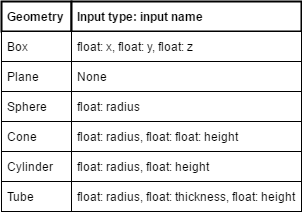
\includegraphics[scale=0.55]{Figures/InputsForGeoms.png}
	\caption{Table of geometric specific inputs for the individual geometries}
	\label{fig:InputsForGeoms}
\end{figure}

Since a lot of transformations are used in the creator it was decided also to create a function to easily create transform objects from R,P,Y and x,y,z values. The function (called getTransform3D) takes in these values and returns a Transform3D object.\\

An example of adding a sphere to a new WorkCell can be seen on figure~\ref{fig:CodeExampleAddSphere}.

\begin{figure}[h]
	\centering
	\lstset{language=C++} 
	\begin{lstlisting}[frame=single]
	// Create new wc
	WorkCell::Ptr dummy = ownedPtr(new WorkCell("wc"));
	 
	// Radius of 10 cm
	float radius = 0.1;
	
	// Displacement of 10 cm in x, y and z
	Transform3D<double> transform = getTransform3D(0.1, 0.1, 0.1, 0, 0, 0); 
	
	// Adding sphere to WorkCell
	ei::creator::addSphere( "testSphere", // Name of Sphere
							"WORLD", // Name of parent frame
							wc, // Pointer to WorkCell
							radius, // Radius of Sphere
							transform); // Transform of Sphere
	 
	\end{lstlisting}
	\caption{Code example of adding a sphere to a new WorkCell. The sphere has a radius of 10 cm and a displacement of 10 cm in x, y and z in relation to the frame on which it is set. The sphere is added to a new movable frame with the parent set to the WORLD frame.}
	\label{fig:CodeExampleAddSphere}
\end{figure}

\subsection{Implementation of the creator}
The creator was implemented with the purpose of using the most upper layers of the RobWork libraries functions to solve as much of the problem as possible. This was done since in RobWork it is possible to access lower levels of the library which makes the RobWork library way more flexible. An example of this could be when working with the frames of a WorkCell the upper layer way of doing it would be accessing the frames through the WorkCell's own functionality for getting frames, whereas the lower layer of doing it would be to access the state structure in the WorkCell and through it access the frames. The other reasoning for using upper layers is that it is usually simpler code, meaning there is less mistakes to make and the mistakes made are easier to find.\\

The implementation of the getTransform3D function is rather simple since it utilises some conversions in the RobWork library. The inputs for the function are 6 doubles representing the x, y, z displacement and the R, P, Y values representing the rotation. In order to create a Transform3D object, a vector representing the displacement and a matrix representing the rotation is needed. The displacement vector is easy to create since it is just a vector containing the values directly from the input. The rotation matrix however is more difficult to get since the input for the rotation is represented in R, P, Y values. The R, P, Y values needs to be converted to a rotation matrix. Instead of doing the calculations manually, RobWork, albeit a little hidden, can do this for us through the RPY class in the math namespace. First an RPY object is created with the values from the input. Then the member function toRotation3D from the RPY class is called returning the rotation matrix of the given R, P, Y values. The displacement vector and rotation matrix is then used to create a Transform3D object that is returned to the user. It would be possible to just implement the same functionality that the toRotation3D RPY class, eliminating the creation of an RPY object. This would increase the computation speed, but not significantly unless the function is used a lot.

\subsubsection{Implementation of creating frames}

\subsubsection{Implementation of creating geometries}
